%
% File emnlp2020.tex
%
%% Based on the style files for ACL 2020, which were
%% Based on the style files for ACL 2018, NAACL 2018/19, which were
%% Based on the style files for ACL-2015, with some improvements
%%  taken from the NAACL-2016 style
%% Based on the style files for ACL-2014, which were, in turn,
%% based on ACL-2013, ACL-2012, ACL-2011, ACL-2010, ACL-IJCNLP-2009,
%% EACL-2009, IJCNLP-2008...
%% Based on the style files for EACL 2006 by 
%%e.agirre@ehu.es or Sergi.Balari@uab.es
%% and that of ACL 08 by Joakim Nivre and Noah Smith

\documentclass[11pt,a4paper]{article}
\usepackage[hyperref]{emnlp2020}
\usepackage{times}
\usepackage{latexsym}
\renewcommand{\UrlFont}{\ttfamily\small}

% ---------------------------------------------------------
% added by me
\usepackage{multirow}
\usepackage{multicol}
\usepackage{caption,subcaption}
\usepackage{calrsfs}
\usepackage{mathrsfs}
\usepackage{graphicx}
\usepackage{algorithm}
\usepackage{algorithmic}
\usepackage[symbol]{footmisc}
\usepackage{url}            % simple URL typesetting
\usepackage{booktabs}       % professional-quality tables
\usepackage{amsfonts}       % blackboard math symbols
\usepackage{nicefrac}       % compact symbols for 1/2, etc.
\usepackage{microtype}      % microtypography
%\usepackage{subfigure}
\usepackage{amsmath,amssymb}
\usepackage{amsfonts}
\usepackage{amsthm}
\usepackage{xspace}
\usepackage{graphicx}
%\input{math_commands.tex}
\usepackage{apxproof}
\usepackage{appendix}
\usepackage{multirow}
\usepackage{multicol}
\usepackage{hyperref}
\usepackage{xcolor}
%% New commands added
\DeclareMathAlphabet{\pazocal}{OMS}{zplm}{m}{n}
\newcommand{\La}{\mathcal{L}}   % curly
\newcommand{\Lb}{\pazocal{L}}   % different
\newcommand{\LD}{\mathfrak{D}}   
% \usepackage{float}
% \usepackage{placeins}
%% New commands ended
\usepackage{amsmath,amsfonts,bm}
\newtheorem{definition}{Definition}[section]
\newtheorem{theorem}{Theorem}
\newtheorem{remark}{Remark}
\newtheorem{proposition}{Proposition}
  
% Mark sections of captions for referring to divisions of figures
\newcommand{\RNum}[1]{\uppercase\expandafter{\romannumeral #1\relax}}
\newcommand{\mb}[1]{\mathbf{#1}}
\newcommand{\mbb}[1]{\mathbb{#1}}
\newcommand{\mc}[1]{\mathcal{#1}}
\newcommand{\tildex}{\tilde{\mb{x}}}
\newcommand{\figleft}{{\em (Left)}}
\newcommand{\figcenter}{{\em (Center)}}
\newcommand{\figright}{{\em (Right)}}
\newcommand{\figtop}{{\em (Top)}}
\newcommand{\figbottom}{{\em (Bottom)}}
\newcommand{\captiona}{{\em (a)}}
\newcommand{\captionb}{{\em (b)}}
\newcommand{\captionc}{{\em (c)}}
\newcommand{\captiond}{{\em (d)}}
\newcommand{\G}{\mathcal{G}}
\newcommand{\N}{\mathcal{N}}
\newcommand{\V}{\mathcal{V}}
% \newcommand{\E}{\mathcal{E}}
\newcommand{\T}{\mathcal{T}}
\newcommand{\A}{\mathcal{A}}
\newcommand{\R}{\mathcal{R}}
\newcommand{\bx}{\mathbf{x}}
\newcommand{\by}{\mathbf{y}}
% Highlight a newly defined term
\newcommand{\newterm}[1]{{\bf #1}}

% Other
\def\defeq{\dot=}
\newcommand\norm[1]{\left\lVert#1\right\rVert} % Norm
\newcommand{\red}{\textcolor{red}}
\DeclareMathOperator*{\argmin}{\arg\!\min}
\DeclareMathOperator*{\hull}{hull}
\DeclareMathOperator*{\argmax}{\arg\!\max}
\newcommand{\xhdr}[1]{{\noindent\bfseries #1}.}
\newcommand{\cut}[1]{}
\newcommand{\CITE}{\textcolor{red}{CITE}}
\newcommand{\joey}[1]{\textcolor{blue}{Joey: #1}}
\newcommand{\removelatexerror}{\let\@latex@error\@gobble}

\usepackage{colortbl}
\definecolor{mistyrose}{rgb}{1.0, 0.89, 0.88}
\definecolor{magicmint}{rgb}{0.67, 0.94, 0.82}
\definecolor{mossgreen}{rgb}{0.68, 0.87, 0.68}
\definecolor{palegreen}{rgb}{0.6, 0.98, 0.6}
\definecolor{pastelgreen}{rgb}{0.47, 0.87, 0.47}
\definecolor{celadon}{rgb}{0.67, 0.88, 0.69}

\usepackage{amsmath,amsfonts,bm}
\newcommand\restr[2]{{% we make the whole thing an ordinary symbol
  \left.\kern-\nulldelimiterspace % automatically resize the bar with \right
  #1 % the function
  \vphantom{\big|} % pretend it's a little taller at normal size
  \right|_{#2} % this is the delimiter
  }}
% Other
\def\defeq{\dot=}
\newcommand{\will}[1]{\textcolor{cyan}{WILL: #1}}


\newcommand{\GNN}{\textsc{GNN}}

% Figure reference, lower-case.
\def\figref#1{figure~\ref{#1}}
% Figure reference, capital. For start of sentence
\def\Figref#1{Figure~\ref{#1}}
\def\twofigref#1#2{figures \ref{#1} and \ref{#2}}
\def\quadfigref#1#2#3#4{figures \ref{#1}, \ref{#2}, \ref{#3} and \ref{#4}}
% Section reference, lower-case.
\def\secref#1{section~\ref{#1}}
% Section reference, capital.
\def\Secref#1{Section~\ref{#1}}
% Reference to two sections.
\def\twosecrefs#1#2{sections \ref{#1} and \ref{#2}}
% Reference to three sections.
\def\secrefs#1#2#3{sections \ref{#1}, \ref{#2} and \ref{#3}}
% Reference to an equation, lower-case.
% \def\eqref#1{equation~\ref{#1}}
% Reference to an equation, upper case
% \def\Eqref#1{Equation~\ref{#1}}
% A raw reference to an equation---avoid using if possible
\def\plaineqref#1{\ref{#1}}
% Reference to a chapter, lower-case.
\def\chapref#1{chapter~\ref{#1}}
% Reference to an equation, upper case.
\def\Chapref#1{Chapter~\ref{#1}}
% Reference to a range of chapters
\def\rangechapref#1#2{chapters\ref{#1}--\ref{#2}}
% Reference to an algorithm, lower-case.
\def\algref#1{algorithm~\ref{#1}}
% Reference to an algorithm, upper case.
\def\Algref#1{Algorithm~\ref{#1}}
\def\twoalgref#1#2{algorithms \ref{#1} and \ref{#2}}
\def\Twoalgref#1#2{Algorithms \ref{#1} and \ref{#2}}
% Reference to a part, lower case
\def\partref#1{part~\ref{#1}}
% Reference to a part, upper case
\def\Partref#1{Part~\ref{#1}}
\def\twopartref#1#2{parts \ref{#1} and \ref{#2}}

\def\ceil#1{\lceil #1 \rceil}
\def\floor#1{\lfloor #1 \rfloor}
\def\1{\bm{1}}
\newcommand{\train}{\mathcal{D}}
\newcommand{\valid}{\mathcal{D_{\mathrm{valid}}}}
\newcommand{\test}{\mathcal{D_{\mathrm{test}}}}

\def\eps{{\epsilon}}


% Random variables
\def\reta{{\textnormal{$\eta$}}}
\def\ra{{\textnormal{a}}}
\def\rb{{\textnormal{b}}}
\def\rc{{\textnormal{c}}}
\def\rd{{\textnormal{d}}}
\def\re{{\textnormal{e}}}
\def\rf{{\textnormal{f}}}
\def\rg{{\textnormal{g}}}
\def\rh{{\textnormal{h}}}
\def\ri{{\textnormal{i}}}
\def\rj{{\textnormal{j}}}
\def\rk{{\textnormal{k}}}
\def\rl{{\textnormal{l}}}
% rm is already a command, just don't name any random variables m
\def\rn{{\textnormal{n}}}
\def\ro{{\textnormal{o}}}
\def\rp{{\textnormal{p}}}
\def\rq{{\textnormal{q}}}
\def\rr{{\textnormal{r}}}
\def\rs{{\textnormal{s}}}
\def\rt{{\textnormal{t}}}
\def\ru{{\textnormal{u}}}
\def\rv{{\textnormal{v}}}
\def\rw{{\textnormal{w}}}
\def\rx{{\textnormal{x}}}
\def\ry{{\textnormal{y}}}
\def\rz{{\textnormal{z}}}

% Random vectors
\def\rvepsilon{{\mathbf{\epsilon}}}
\def\rvtheta{{\mathbf{\theta}}}
\def\rva{{\mathbf{a}}}
\def\rvb{{\mathbf{b}}}
\def\rvc{{\mathbf{c}}}
\def\rvd{{\mathbf{d}}}
\def\rve{{\mathbf{e}}}
\def\rvf{{\mathbf{f}}}
\def\rvg{{\mathbf{g}}}
\def\rvh{{\mathbf{h}}}
\def\rvu{{\mathbf{i}}}
\def\rvj{{\mathbf{j}}}
\def\rvk{{\mathbf{k}}}
\def\rvl{{\mathbf{l}}}
\def\rvm{{\mathbf{m}}}
\def\rvn{{\mathbf{n}}}
\def\rvo{{\mathbf{o}}}
\def\rvp{{\mathbf{p}}}
\def\rvq{{\mathbf{q}}}
\def\rvr{{\mathbf{r}}}
\def\rvs{{\mathbf{s}}}
\def\rvt{{\mathbf{t}}}
\def\rvu{{\mathbf{u}}}
\def\rvv{{\mathbf{v}}}
\def\rvw{{\mathbf{w}}}
\def\rvx{{\mathbf{x}}}
\def\rvy{{\mathbf{y}}}
\def\rvz{{\mathbf{z}}}

% Elements of random vectors
\def\erva{{\textnormal{a}}}
\def\ervb{{\textnormal{b}}}
\def\ervc{{\textnormal{c}}}
\def\ervd{{\textnormal{d}}}
\def\erve{{\textnormal{e}}}
\def\ervf{{\textnormal{f}}}
\def\ervg{{\textnormal{g}}}
\def\ervh{{\textnormal{h}}}
\def\ervi{{\textnormal{i}}}
\def\ervj{{\textnormal{j}}}
\def\ervk{{\textnormal{k}}}
\def\ervl{{\textnormal{l}}}
\def\ervm{{\textnormal{m}}}
\def\ervn{{\textnormal{n}}}
\def\ervo{{\textnormal{o}}}
\def\ervp{{\textnormal{p}}}
\def\ervq{{\textnormal{q}}}
\def\ervr{{\textnormal{r}}}
\def\ervs{{\textnormal{s}}}
\def\ervt{{\textnormal{t}}}
\def\ervu{{\textnormal{u}}}
\def\ervv{{\textnormal{v}}}
\def\ervw{{\textnormal{w}}}
\def\ervx{{\textnormal{x}}}
\def\ervy{{\textnormal{y}}}
\def\ervz{{\textnormal{z}}}

% Random matrices
\def\rmA{{\mathbf{A}}}
\def\rmB{{\mathbf{B}}}
\def\rmC{{\mathbf{C}}}
\def\rmD{{\mathbf{D}}}
\def\rmE{{\mathbf{E}}}
\def\rmF{{\mathbf{F}}}
\def\rmG{{\mathbf{G}}}
\def\rmH{{\mathbf{H}}}
\def\rmI{{\mathbf{I}}}
\def\rmJ{{\mathbf{J}}}
\def\rmK{{\mathbf{K}}}
\def\rmL{{\mathbf{L}}}
\def\rmM{{\mathbf{M}}}
\def\rmN{{\mathbf{N}}}
\def\rmO{{\mathbf{O}}}
\def\rmP{{\mathbf{P}}}
\def\rmQ{{\mathbf{Q}}}
\def\rmR{{\mathbf{R}}}
\def\rmS{{\mathbf{S}}}
\def\rmT{{\mathbf{T}}}
\def\rmU{{\mathbf{U}}}
\def\rmV{{\mathbf{V}}}
\def\rmW{{\mathbf{W}}}
\def\rmX{{\mathbf{X}}}
\def\rmY{{\mathbf{Y}}}
\def\rmZ{{\mathbf{Z}}}

% Elements of random matrices
\def\ermA{{\textnormal{A}}}
\def\ermB{{\textnormal{B}}}
\def\ermC{{\textnormal{C}}}
\def\ermD{{\textnormal{D}}}
\def\ermE{{\textnormal{E}}}
\def\ermF{{\textnormal{F}}}
\def\ermG{{\textnormal{G}}}
\def\ermH{{\textnormal{H}}}
\def\ermI{{\textnormal{I}}}
\def\ermJ{{\textnormal{J}}}
\def\ermK{{\textnormal{K}}}
\def\ermL{{\textnormal{L}}}
\def\ermM{{\textnormal{M}}}
\def\ermN{{\textnormal{N}}}
\def\ermO{{\textnormal{O}}}
\def\ermP{{\textnormal{P}}}
\def\ermQ{{\textnormal{Q}}}
\def\ermR{{\textnormal{R}}}
\def\ermS{{\textnormal{S}}}
\def\ermT{{\textnormal{T}}}
\def\ermU{{\textnormal{U}}}
\def\ermV{{\textnormal{V}}}
\def\ermW{{\textnormal{W}}}
\def\ermX{{\textnormal{X}}}
\def\ermY{{\textnormal{Y}}}
\def\ermZ{{\textnormal{Z}}}

% Vectors
\def\vzero{{\bm{0}}}
\def\vone{{\bm{1}}}
\def\vmu{{\bm{\mu}}}
\def\vtheta{{\bm{\theta}}}
\def\va{{\bm{a}}}
\def\vb{{\bm{b}}}
\def\vc{{\bm{c}}}
\def\vd{{\bm{d}}}
\def\ve{{\bm{e}}}
\def\vf{{\bm{f}}}
\def\vg{{\bm{g}}}
\def\vh{{\bm{h}}}
\def\vi{{\bm{i}}}
\def\vj{{\bm{j}}}
\def\vk{{\bm{k}}}
\def\vl{{\bm{l}}}
\def\vm{{\bm{m}}}
\def\vn{{\bm{n}}}
\def\vo{{\bm{o}}}
\def\vp{{\bm{p}}}
\def\vq{{\bm{q}}}
\def\vr{{\bm{r}}}
\def\vs{{\bm{s}}}
\def\vt{{\bm{t}}}
\def\vu{{\bm{u}}}
\def\vv{{\bm{v}}}
\def\vw{{\bm{w}}}
\def\vx{{\bm{x}}}
\def\vy{{\bm{y}}}
\def\vz{{\bm{z}}}

% Elements of vectors
\def\evalpha{{\alpha}}
\def\evbeta{{\beta}}
\def\evepsilon{{\epsilon}}
\def\evlambda{{\lambda}}
\def\evomega{{\omega}}
\def\evmu{{\mu}}
\def\evpsi{{\psi}}
\def\evsigma{{\sigma}}
\def\evtheta{{\theta}}
\def\eva{{a}}
\def\evb{{b}}
\def\evc{{c}}
\def\evd{{d}}
\def\eve{{e}}
\def\evf{{f}}
\def\evg{{g}}
\def\evh{{h}}
\def\evi{{i}}
\def\evj{{j}}
\def\evk{{k}}
\def\evl{{l}}
\def\evm{{m}}
\def\evn{{n}}
\def\evo{{o}}
\def\evp{{p}}
\def\evq{{q}}
\def\evr{{r}}
\def\evs{{s}}
\def\evt{{t}}
\def\evu{{u}}
\def\evv{{v}}
\def\evw{{w}}
\def\evx{{x}}
\def\evy{{y}}
\def\evz{{z}}

% Matrix
\def\mA{{\bm{A}}}
\def\mB{{\bm{B}}}
\def\mC{{\bm{C}}}
\def\mD{{\bm{D}}}
\def\mE{{\bm{E}}}
\def\mF{{\bm{F}}}
\def\mG{{\bm{G}}}
\def\mH{{\bm{H}}}
\def\mI{{\bm{I}}}
\def\mJ{{\bm{J}}}
\def\mK{{\bm{K}}}
\def\mL{{\bm{L}}}
\def\mM{{\bm{M}}}
\def\mN{{\bm{N}}}
\def\mO{{\bm{O}}}
\def\mP{{\bm{P}}}
\def\mQ{{\bm{Q}}}
\def\mR{{\bm{R}}}
\def\mS{{\bm{S}}}
\def\mT{{\bm{T}}}
\def\mU{{\bm{U}}}
\def\mV{{\bm{V}}}
\def\mW{{\bm{W}}}
\def\mX{{\bm{X}}}
\def\mY{{\bm{Y}}}
\def\mZ{{\bm{Z}}}
\def\mBeta{{\bm{\beta}}}
\def\mPhi{{\bm{\Phi}}}
\def\mLambda{{\bm{\Lambda}}}
\def\mSigma{{\bm{\Sigma}}}

% Tensor
\DeclareMathAlphabet{\mathsfit}{\encodingdefault}{\sfdefault}{m}{sl}
\SetMathAlphabet{\mathsfit}{bold}{\encodingdefault}{\sfdefault}{bx}{n}
\newcommand{\tens}[1]{\bm{\mathsfit{#1}}}
\def\tA{{\tens{A}}}
\def\tB{{\tens{B}}}
\def\tC{{\tens{C}}}
\def\tD{{\tens{D}}}
\def\tE{{\tens{E}}}
\def\tF{{\tens{F}}}
\def\tG{{\tens{G}}}
\def\tH{{\tens{H}}}
\def\tI{{\tens{I}}}
\def\tJ{{\tens{J}}}
\def\tK{{\tens{K}}}
\def\tL{{\tens{L}}}
\def\tM{{\tens{M}}}
\def\tN{{\tens{N}}}
\def\tO{{\tens{O}}}
\def\tP{{\tens{P}}}
\def\tQ{{\tens{Q}}}
\def\tR{{\tens{R}}}
\def\tS{{\tens{S}}}
\def\tT{{\tens{T}}}
\def\tU{{\tens{U}}}
\def\tV{{\tens{V}}}
\def\tW{{\tens{W}}}
\def\tX{{\tens{X}}}
\def\tY{{\tens{Y}}}
\def\tZ{{\tens{Z}}}


% Graph
\def\gA{{\mathcal{A}}}
\def\gB{{\mathcal{B}}}
\def\gC{{\mathcal{C}}}
\def\gD{{\mathcal{D}}}
\def\gE{{\mathcal{E}}}
\def\gF{{\mathcal{F}}}
\def\gG{{\mathcal{G}}}
\def\gH{{\mathcal{H}}}
\def\gI{{\mathcal{I}}}
\def\gJ{{\mathcal{J}}}
\def\gK{{\mathcal{K}}}
\def\gL{{\mathcal{L}}}
\def\gM{{\mathcal{M}}}
\def\gN{{\mathcal{N}}}
\def\gO{{\mathcal{O}}}
\def\gP{{\mathcal{P}}}
\def\gQ{{\mathcal{Q}}}
\def\gR{{\mathcal{R}}}
\def\gS{{\mathcal{S}}}
\def\gT{{\mathcal{T}}}
\def\gU{{\mathcal{U}}}
\def\gV{{\mathcal{V}}}
\def\gW{{\mathcal{W}}}
\def\gX{{\mathcal{X}}}
\def\gY{{\mathcal{Y}}}
\def\gZ{{\mathcal{Z}}}

% Sets
\def\sA{{\mathbb{A}}}
\def\sB{{\mathbb{B}}}
\def\sC{{\mathbb{C}}}
\def\sD{{\mathbb{D}}}
% Don't use a set called E, because this would be the same as our symbol
% for expectation.
\def\sF{{\mathbb{F}}}
\def\sG{{\mathbb{G}}}
\def\sH{{\mathbb{H}}}
\def\sI{{\mathbb{I}}}
\def\sJ{{\mathbb{J}}}
\def\sK{{\mathbb{K}}}
\def\sL{{\mathbb{L}}}
\def\sM{{\mathbb{M}}}
\def\sN{{\mathbb{N}}}
\def\sO{{\mathbb{O}}}
\def\sP{{\mathbb{P}}}
\def\sQ{{\mathbb{Q}}}
\def\sR{{\mathbb{R}}}
\def\sS{{\mathbb{S}}}
\def\sT{{\mathbb{T}}}
\def\sU{{\mathbb{U}}}
\def\sV{{\mathbb{V}}}
\def\sW{{\mathbb{W}}}
\def\sX{{\mathbb{X}}}
\def\sY{{\mathbb{Y}}}
\def\sZ{{\mathbb{Z}}}

% Entries of a matrix
\def\emLambda{{\Lambda}}
\def\emA{{A}}
\def\emB{{B}}
\def\emC{{C}}
\def\emD{{D}}
\def\emE{{E}}
\def\emF{{F}}
\def\emG{{G}}
\def\emH{{H}}
\def\emI{{I}}
\def\emJ{{J}}
\def\emK{{K}}
\def\emL{{L}}
\def\emM{{M}}
\def\emN{{N}}
\def\emO{{O}}
\def\emP{{P}}
\def\emQ{{Q}}
\def\emR{{R}}
\def\emS{{S}}
\def\emT{{T}}
\def\emU{{U}}
\def\emV{{V}}
\def\emW{{W}}
\def\emX{{X}}
\def\emY{{Y}}
\def\emZ{{Z}}
\def\emSigma{{\Sigma}}

% entries of a tensor
% Same font as tensor, without \bm wrapper
\newcommand{\etens}[1]{\mathsfit{#1}}
\def\etLambda{{\etens{\Lambda}}}
\def\etA{{\etens{A}}}
\def\etB{{\etens{B}}}
\def\etC{{\etens{C}}}
\def\etD{{\etens{D}}}
\def\etE{{\etens{E}}}
\def\etF{{\etens{F}}}
\def\etG{{\etens{G}}}
\def\etH{{\etens{H}}}
\def\etI{{\etens{I}}}
\def\etJ{{\etens{J}}}
\def\etK{{\etens{K}}}
\def\etL{{\etens{L}}}
\def\etM{{\etens{M}}}
\def\etN{{\etens{N}}}
\def\etO{{\etens{O}}}
\def\etP{{\etens{P}}}
\def\etQ{{\etens{Q}}}
\def\etR{{\etens{R}}}
\def\etS{{\etens{S}}}
\def\etT{{\etens{T}}}
\def\etU{{\etens{U}}}
\def\etV{{\etens{V}}}
\def\etW{{\etens{W}}}
\def\etX{{\etens{X}}}
\def\etY{{\etens{Y}}}
\def\etZ{{\etens{Z}}}

% ---------------------------------------------------------



% This is not strictly necessary, and may be commented out,
% but it will improve the layout of the manuscript,
% and will typically save some space.
\usepackage{microtype}
% \aclfinalcopy % Uncomment this line for the final submission
%\def\aclpaperid{***} %  Enter the acl Paper ID here

%\setlength\titlebox{5cm}
% You can expand the titlebox if you need extra space
% to show all the authors. Please do not make the titlebox
% smaller than 5cm (the original size); we will check this
% in the camera-ready version and ask you to change it back.

\newcommand\BibTeX{B\textsc{ib}\TeX}

\title{Structure Aware Negative Sampling in Knowledge Graphs}

\author{Kian Ahrabian\thanks{$\text{\;}$ Equal contribution}$^{\text{\; },1,3}$, Aarash Feizi\footnotemark[1]$^{\text{\; },1,3}$, Yasmin Salehi\footnotemark[1]$^{\text{\; },2}$, \\ {\bf William L. Hamilton$^{1,3}$} \and {\bf Avishak Joey Bose$^{1,3}$} \\ 
$^1$ School of Computer Science, McGill University, Canada \\
$^2$ Department of Electrical and Computer Engineering, McGill University, Canada \\
$^3$ Montreal Institute of Learning Algorithms (Mila), Canada \\
\{\texttt{kian.ahrabian}, \texttt{aarash.feizi}, \texttt{yasmin.salehi}, \texttt{wlh}, \texttt{joey.bose} \} \\
\{\texttt{@mail.mcgill.ca}, \texttt{@mail.mcgill.ca}, \texttt{@mail.mcgill.ca}, \\ \texttt{@cs.mcgill.ca}, \texttt{@mail.mcgill.ca} \}
}

\date{}

\begin{document}
\maketitle
\begin{abstract}
Contrastive estimation is the most predominantly used technique for learning low dimensional knowledge graph (KG) representations for eliminating the computational burdens associated with calculating the normalization constant in softmax prediction layers. Given that KGs only consist of facts benefiting from this approach necessitates the fabrication of negative samples. Therefore, a crucial aspect of training KG embeddings is the choice of negative sampling distribution, which balances computational complexity of intractable objectives with hard negatives. While, earlier methods either employ too simple distributions, i.e. uniform, or sophisticated adversarial distributions they do not explicitly incorporate known graph structure resulting in suboptimal negatives. In this paper, we propose Structure Aware Negative Sampling (SANS), a computationally cheap negative sampling strategy that utilizes the rich graph structure by selecting negative samples from a node's \emph{k-hop} neighbourhood. We also employ a dynamic sampling scheme which results in significantly harder negatives than uniform sampling, yet is computationally cheaper than state-of-the-art approaches while producing competitive results. 



% Version 3 ----------------------------------------------------------------------------------

\cut{
Learning low dimensional representations for entities and relations in knowledge graphs (KGs) represents a scalable and effective method for inferring connectivity patterns and predicting missing links. Since KGs consist of only positive facts, negative samples (false relations) are required for contrastive estimation during training. Therefore, a crucial aspect of training KG embeddings is the choice of negative sampling (NEG) distribution, which balances computational complexity of intractable objectives with hard negatives. While, earlier methods either employ too simple distributions, i.e. uniform, or sophisticated adversarial distributions they do not explicitly incorporate known graph structure resulting in suboptimal negatives. In this paper, we propose Structure Aware Negative Sampling (SANS), a computationally cheap negative sampling strategy that utilizes the rich graph structure by selecting negative samples from a node's \emph{k-hop} neighbourhood. We also employ a dynamic sampling scheme which results in significantly harder negatives than uniform sampling, yet is computationally cheaper than state-of-the-art approaches while producing competitive results. 
}

% Version 2 ----------------------------------------------------------------------------------
\cut{
Learning low dimensional representations for entities and relations in knowledge graphs (KGs) represents a scalable and effective method for inferring connectivity patterns and predicting missing links. A crucial aspect of training KG embeddings is the choice of negative sampling (NEG) distribution, which balances computational complexity of intractable objectives with hard negatives. While, earlier methods either employ too simple distributions, i.e. uniform, or sophisticated adversarial distributions they do not explicitly incorporate known graph structure resulting in suboptimal negatives.
In this paper, we propose Structure Aware Negative Sampling (SANS), a computationally cheap NEG strategy that utilizes the rich graph structure by selecting negative samples from a node's \emph{k-hop} neighbourhood. We also employ a dynamic sampling scheme which results in significantly harder negatives than uniform sampling, yet is computationally cheaper than state of the art approaches while producing competitive results. 
}

% Version 1 ----------------------------------------------------------------------------------
\cut{
Considering that KGs only consist of observed true facts, effective negative sampling (NEG) is an important aspect while training graph embedding models. Earlier methods for performing NEG assumed simple distributions, ---i.e. uniform, for negative triples during training, resulting in poor training of the KG embedding model due to easily-classified negative examples that provided little information alongside the positive examples. In this work, we select the negative triples from the node's \emph{k-hop} neighbourhood, and we propose a dynamic sampling scheme. With respect to our obtained results, our NEG technique performs better than uniform sampling, yet uses less computational resources compared to some of the state-of-the-art NEG algorithms.
}



\end{abstract}

\section{Introduction}

Knowledge Graphs represent repositories of information organized as factual triples ($h,r,t$), where head and tail entities are connected via a particular a relation ($r$). Indeed, KGs have seen wide application in a variety of domains from question answering \cite{yao2014information, malinowski2014multi, hao2017end}, natural language processing \cite{berant2013semantic, yu2014improving, yang2019leveraging} to name a few. While often large and expansive, real world KGs such as FreeBase \cite{bollacker2008freebase} and WordNet \cite{miller1995wordnet} are known to be incomplete. Consequently, KG completion via link prediction constitutes a fundamental task \cite{sun2019rotate, kotnis2017analysis, angeli2013philosophers}.

In recent years, there has been a surge of methods employing graph embedding techniques that encode KGs into a lower-dimensional vector space facilitating easier data manipulation \cite{zhang2019nscaching}, while being an attractive framework for handling data sparsity and incompleteness \cite{wang2018incorporating}. To ease computational burdens associated with training KG's embedding models, contrastive estimation \cite{gutmann2010noise} has emerged as the defacto gold standard allowing for the efficient scaling of models to large datasets; it solely trains the model with real data (positive samples) and noise (negative samples) distributions \cite{ma2018noise}. Leveraging contrastive estimation to train KG embedding models thus involves optimizing the model to maximize the score of positive triplets and minimize the score of negative triplets, where score is calculated by the decoder function. %\footnote{Viewing KG embedding models from an encoder-decoder perspective, an encoder maps the nodes into a lower dimensional space while a decoder reconstructs information about a node’s neighborhood from the node’s embedding \cite{hamilton2017representation}.}.

It has been observed that the choice of negative sample distribution plays a crucial role as simple random sampling ---i.e. NCE \cite{gutmann2010noise}, produces negatives that are easily classified and provide little information alongside the observed positive examples \cite{zhang2019nscaching, wang2018incorporating}. Such negative triplets are associated with small scores which impede the optimization process in early stages of training. 
There exists many approaches that seek to learn a more complex negative sampling distribution, such as adversarial samplers \cite{cai2017kbgan, bose2018adversarial}, Self-Adversarial NEG \cite{sun2019rotate}, or even refining the sampling process by using cached high quality negative triplets \cite{zhang2019nscaching}. However, adversarial negative sampling approaches are computationally expensive, while more tractable approaches (e.g., based on caches) tend to ignore the rich graph structure available in KGs. This raises the question of whether we can find a computationally inexpensive negative sampling strategy that can still leverage the rich graph structure of KGs.

%----------------------------------------------------------
%----------------------------------------------------------
% Start of previous versions
\cut{
In recent years, there has been a surge of methods employing graph embedding techniques that encode KGs into a lower-dimensional vector space facilitating easier data manipulation \cite{zhang2019nscaching}, while being an attractive framework for handling data sparsity and incompleteness \cite{wang2018incorporating}. To ease computational burdens associated with training KG's embedding models, negative sampling \CITE has emerged as the defacto gold standard allowing for the efficient scaling of models to large datasets. It has been observed that the choice of (NEG) distribution plays a crucial role as simple random sampling ---i.e. NCE \cite{gutmann2010noise}, produces easy negatives that are easily classified and provide little information alongside the observed positive examples \cite{zhang2019nscaching,wang2018incorporating}. While there exists many approaches that seek to learn a more complex (NEG) distribution, such as adversarial samplers \cite{cai2017kbgan, bose2018adversarial}, Self-Adversarial NEG \cite{sun2019rotate}, or even refining the sampling process by using cached high quality negative triplets \cite{zhang2019nscaching} none explicitly use the rich graph structure directly available in a KG. Can we find a computationally inexpensive NEG distribution that provides high quality hard negatives by directly utilizing graph structure?
}

\cut{
Knowledge Graphs (KGs) are knowledge bases that store and represent information using graph structure, where a relation ($r$) between two entities, namely the head ($h$) and tail ($t$) entities, is denoted as $(h,r,t)$. FreeBase \cite{bollacker2008freebase} and WordNet \cite{miller1995wordnet} are two examples of real-world KGs, which have applications in question answering \cite{yao2014information, malinowski2014multi, hao2017end}, natural language processing \cite{berant2013semantic, yu2014improving, yang2019leveraging}, and many other domains. 

Regardless of containing a significant amount of information, KGs tend to often become incomplete as their domain gets larger, since collecting all possible relations becomes practically infeasible \cite{sun2019rotate,kotnis2017analysis,angeli2013philosophers}. Therefore, knowledge graph completion has turned into a fundamental task when studying KGs, which intends to infer the missing links or the probability of correctness of the existing ones \cite{angeli2013philosophers}. In this regard, recent years have seen a surge of research on graph embedding techniques aiming to encode KGs into a lower-dimensional vector space to facilitate data manipulation \cite{zhang2019nscaching}, and provide a numerical and computational framework for handling data sparsity as well as incompleteness \cite{wang2018incorporating}. 

While training KG embeddings, Negative Sampling (NEG) is an integral part to the learning process as KGs only include positive triples \cite{zhang2019nscaching,trouillon2016complex}. In the literature, early work used uniform sampling to obtain negative triples for training their graph embedding models \cite{wang2017knowledge,bordes2013translating}. While simple, such NEG technique is a fixed scheme and ignores the varying distribution of negative triplets during training, which results in picking negative samples that do not provide any meaningful information \cite{zhang2019nscaching,wang2018incorporating,cai2017kbgan}. Consequently, other techniques were proposed to tackle this issue by choosing negative examples more effectively, some of which involve leveraging Generative Adversarial Networks (GANs) \cite{goodfellow2014generative}, Self-Adversarial NEG \cite{sun2019rotate}, or refining the sampling process by sampling from cached high quality negative triplets \cite{zhang2019nscaching}. 
}

% End of previous versions 
% ----------------------------------------------------------
% ----------------------------------------------------------

\xhdr{Present Work}
In this work, we seek to find hard negative examples to train a KG embedding model by directly using explicit graph structure in the form of an entity's $\emph{k-hop}$ neighborhood. We hypothesize that entities that are within each other's neighbourhood but share no direct relation have higher chances of being related to one another and thus are good candidates for negative sampling. We argue that such local negatives are harder to distinguish and lead to high scores evaluated by the embedding model. We term our approach \emph{Structure Aware Negative Sampling} (SANS), depicted in Fig. \ref{fig:arch}, as it utilizes the underlying graph structure. Our approach, while being algorithmically simple, enjoys inexpensive generation of high quality negatives at inference time. Empirically, we find that negative sampling using SANS consistently leads to higher scores in MRR and Hit@10 over uniform sampling and competitive scores against sophisticated adversarial samplers at a fraction of the computational cost in two representative KG benchmarks and three score functions. 

\cut{
Inspired by GAN-based and cache-based approaches, which all aim to select high-quality negative triplets, in this work, the effect of generating negative samples with respect to nodes' neighbourhood is investigated, hence why our proposed approach is called \emph{Structural Negative Sampling}. The heuristic used while performing sampling is that nodes that are within each other's neighbourhood have higher chances of being related to one another. In this regard, two nodes that are in the same neighbourhood of an arbitrary distance $r$ that are not connected can make a negative triplet that has a high score (evaluated from the embedding model score functions) and is of high quality. Therefore, not only our proposed NEG scheme benefits from using the underlying graph structure, it is also simple and inexpensive to train yet effective. This idea is analogous to how negative triplets are generated in DeepWalk \cite{perozzi2014deepwalk} and node2vec \cite{grover2016node2vec}, in which the node degree or word frequency is considered respectively. A high-level architectural diagram of our proposed NEG scheme is shown in Figure \ref{fig:arch}.
}
\begin{figure}
    \centering
    
\includegraphics[width=3in]{writeup/archfig.png}
    \caption{Our proposed approach for training a graph embedding model. In this illustration, $k$ is set to $2$.}
    \label{fig:arch}
\end{figure}

% The rest of this paper is structured as follows. Section \ref{sec:relatedwork} provides an overview of related work. Section \ref{sec:proposedapproach} discusses the proposed structural NEG algorithm. Section \ref{sec:exp} presents the experimental setup and the evaluation protocols used alongside the baselines considered. Section \ref{sec:results} presents the results. Finally, concluding remarks and future directions are given in Section \ref{sec:conclusion}. 


% Section \ref{sec:background} provides background knowledge on different knowledge graph embedding models, and how they are trained with negative samples. 



\section{Background and Related Work}
\label{sec:background}
\xhdr{Negative Sampling} 
To address the computational intractability of scaling log-linear models, especially in the context of word and graph embeddings \cite{mikolov2013distributed}, negative sampling can be used. The key idea is to avoid the expensive normalization constant in computing the softmax by training a model to distinguish between observed positive data and fictitious negative examples that are generated by corrupting the positive examples. This general approach is a simplification of the noise contrastive estimation framework \cite{gutmann2010noise}, which is based on Monte-Carlo approximation used in Importance Sampling (IS) \cite{bengio2003quick}, where samples are taken from a distribution that is a mixture of training and noise distributions. 

Given an observed positive triplet $(h,r,t)$ a negative sample can be constructed by corrupting either the head or tail entity to form a new triplet ---i.e. $(h',r,t')$, where either $h',t' \in E$, where $E$ is the set of all entities in the KG.
\cut{
\begin{equation}
    (h',r,t') = \{ (h',r,t)|h'\in E\} \cup \{(h,r,t')|t'\in E \}  \\
\end{equation}
}
Additionally, we assume that the graph embedding models are using a loss function of the following form:
\begin{align}
    \Lb = &\sum_{(h,r,t) \in S} -\text{log }\sigma(\gamma - d_{r}(\boldsymbol{h},\boldsymbol{t}))  \notag \\ 
    - &\sum_{i=1}^{k} \frac{1}{k}\text{log }\sigma(d_r(\boldsymbol{h}_i^{'},\boldsymbol{t}_i^{'})-\gamma)
\end{align}
where $d_r(h,t)$ denotes the score assigned to the compatibility of head and tail entities under the relation $r$, $\gamma$ is a fixed margin, $\sigma$ is the sigmoid function, and $k$ is the number of negative samples.

% ----------------------------------------------------------------------------------------------------------------------------------------------------------------------------------
\xhdr{Non-Fixed Negative Sampling}
\label{sec:relatedwork}
As proposed in \cite{mikolov2013distributed}, negative triplets can be generated using a uniform sampling scheme. However, such uniform and fixed sampling scheme results in easily-classified negative triplets during training, which do not provide any meaningful information \cite{sun2019rotate, zhang2019nscaching}. Consequently, as the training progresses, most of the sampled negative triplets receive small scores and almost zero gradient, impeding the training of the graph embedding model after only a small number of iterations. 

To address the issue of easy negatives, ~\citet{sun2019rotate} propose Self-Adversarial negative sampling, which weighs each sampled negative according its probability under the embedding model. Alternatively, the authors in \cite{wang2018incorporating} and \cite{cai2017kbgan} try creating high quality negative samples by exploiting Generative Adversarial Networks (GANs) \cite{goodfellow2014generative}. Although effective, GAN-based sampling schemes are expensive to train and require gradient estimation techniques, ---i.e. REINFORCE \cite{williams1992simple} , whose variance can scale linearly with the size of $E$ \cite{cai2017kbgan}. Another, elegant approach to hard negative mining involves using a cache of high-quality negative triplets ---i.e. those with high scores \cite{zhang2019nscaching}. In comparison to the GAN-based methods, NSCaching uses considerably less parameters and is easier to train. 

 

\cut{
To overcome the limitations of GAN-based negative sampling methods, ~\citet{zhang2019nscaching} propose a negative sampling approach based on a cache, named NSCaching using which a set of high-quality negative triplets (those with high scores) is maintained and negative triples are sampled from. In comparison to the GAN-based methods, NSCaching uses considerably less parameters and is easier to train. }




\section{Proposed Approach}
\label{sec:proposedapproach}
In this paper, we seek to explicitly use the rich graph structure surrounding a particular node when generating negative triplets. We motivate our approach based on the observation that prior work in learning word embeddings \cite{mikolov2013distributed}, where negative sampling has historically developed, lacked the richness of graph structure that is immediately accessible in the KG setting. Consequently, we hypothesize that enriching the negative sampling process with structural information in KG can yield harder negative examples, crucial to learning of effective embeddings. The preliminary step for implementing this idea is building the k-hop neighbourhood ($K$) of each node, which can be computed using the formula below: 
\begin{equation}
\label{eqn:khop}
K = A^{k} + A^{k-1}
\end{equation}
for $k>0$, where $k$ is an arbitrary number, representing the desired neighbourhood radius to be considered during sampling for a given centre node, and $A$ stands for \emph{adjacency matrix}. 

\cut{ However, since computing Eq. \ref{eqn:khop} can be costly for large KG's due to matrix multiplication, the \emph{k-hop} neighbourhood can be approximated using \emph{Random Walks (RW)} \cite{perozzi2014deepwalk} by Algorithm \ref{alg:rw}, where $\omega$ is the number of RWs, and $k$ is the number of k-hops.

\begin{algorithm}[tb]
   \caption{\small Approximating K-hop neighbourhood using RWs}
   \label{alg:rw}
  \begin{small}
\begin{algorithmic}
   \STATE {\bfseries Input:} $A, k, \omega$
   \COMMENT A: Adjacency Matrix, k: \# of k-hops, $\omega$: \# of RWs
   \STATE {$K \gets$ sparseMatrix($|A| \times |A|$)}
   \FORALL {entity $e$}
   \STATE {$K[e] \gets $} randomWalk(k, $\omega$)
   \ENDFOR
   \STATE {\textbf{return}} $K$
\end{algorithmic}
\end{small}
\end{algorithm}
}
Consequently, given a value for $k$, the \emph{k-hop} neighbourhood of an entity (node) within the graph is calculated, and the negative triples are made by selecting the head $h$ or tail $t$ entity from the \emph{k-hop} neighbourhood that satisfy this criterion:
\begin{equation}
    (h',r,t') = \{ (h',r,t)|h'\in K\} \cup \{(h,r,t')|t'\in K \}  \\
\end{equation}
with $ K \subset E$, where $K$ is the \emph{k-hop} neighbourhood of $h$ or $t$, and $E$ is the entire sample space. It should be noted that since different relation types are considered in our sampling scheme, an additional dimension is added to the adjacency (A) and \emph{k-hop} (K) matrices, resulting in adjacency and \emph{k-hop} tensors.

\subsection{Variants of SANS}

We can also extend the self-adversarial approach in \cite{sun2019rotate} using the SANS approach by restricting the negative triplet distribution in Eq.\ref{eq:dist_adv} to the \emph{k-hop} neighbourhood. In the subsequent sections, we refer to this technique as \emph{Self-Adversarial SANS}, whereas the former approach is referred to as \emph{Uniform SANS}. 


\section{Experiments}
\label{sec:results}

\subsection{Experimental Setting}
% Dataset and evaluation metrics

To conduct experiments for our proposed methods, datasets FB15K-237, which is a variant of FB15K \cite{bollacker2008freebase}, as well as WN18 \cite{miller1995wordnet} are used. For evaluation, our results will be achieved by training the TransE, DistMult, and RotatE models, during which the train set triplets consist of positive triplets $(h , r, t)$ as well as negative triplets, $(h', r, t')$. To evaluate the impact of our NEG schemes on the learned embedding, Hits at N (H@N),  Mean Rank (MR), and Mean Reciprocal Rank (MRR) are used as evaluation measures. 

% Hyperparameter and baseline

For the negative sampling step, $k$ is the main hyperparameter which determines the \emph{k-hop} neighbourhood of each entity. 
% ------------------------------------------------------
% Remove start
\cut{
Furthermore, another important hyperparameter in our scheme is the number of random walks, denoted as $\omega$, when \emph{Random Walks} is being used to approximate the \emph{k-hop} neighbourhood. }
% Remove end
% ------------------------------------------------------

Lastly, our baselines are the results achieved after training the same graph embedding model combined with uniform NEG, and Self-Adversarial NEG, as done in \cite{sun2019rotate}. The hyperparameters that yield the best performance of graph embedding models on the validation set can be found in Section \ref{sec:supplemental}.

\subsection{Results}

% Our most important findings
    % we beat uniform baseline 
    % we need 3500 RW to approximate the adjacency tensor 
    % our matrices are sparse according to table 3
    % We observe that a relatively small subset of nodes ---i.e. 26%, are needed to achieve competitive performance with SOTA methods reaffirming our original hypothesis local negatives in KG's provide a useful learning signal.

\cut{
To infer the number of random walks which can adequately approximate the k-hop tensor, we investigated the effect of different numbers of random walks, $\omega$, ranging from 100 to 3000 illustrated in Figure \ref{fig:ablation}. In these graphs, two baselines are exhibited, namely the one representing the output when negative sampling was done uniformly, and the other being our best performance achieved by our Uniform SANS combined with TransE, for which the k-hop tensor was explicitly computed. According to our observations, our model beats both baselines when the k-hop tensor is approximated with 3000 random walks. This result can be justified by acknowledging that the nodes’ indices that are within close proximity in the k-hop tensor will have larger values; this will yield a weighted negative sampling scheme and may be the contributor to the increased performance.

\begin{figure}[h]
    \centering
    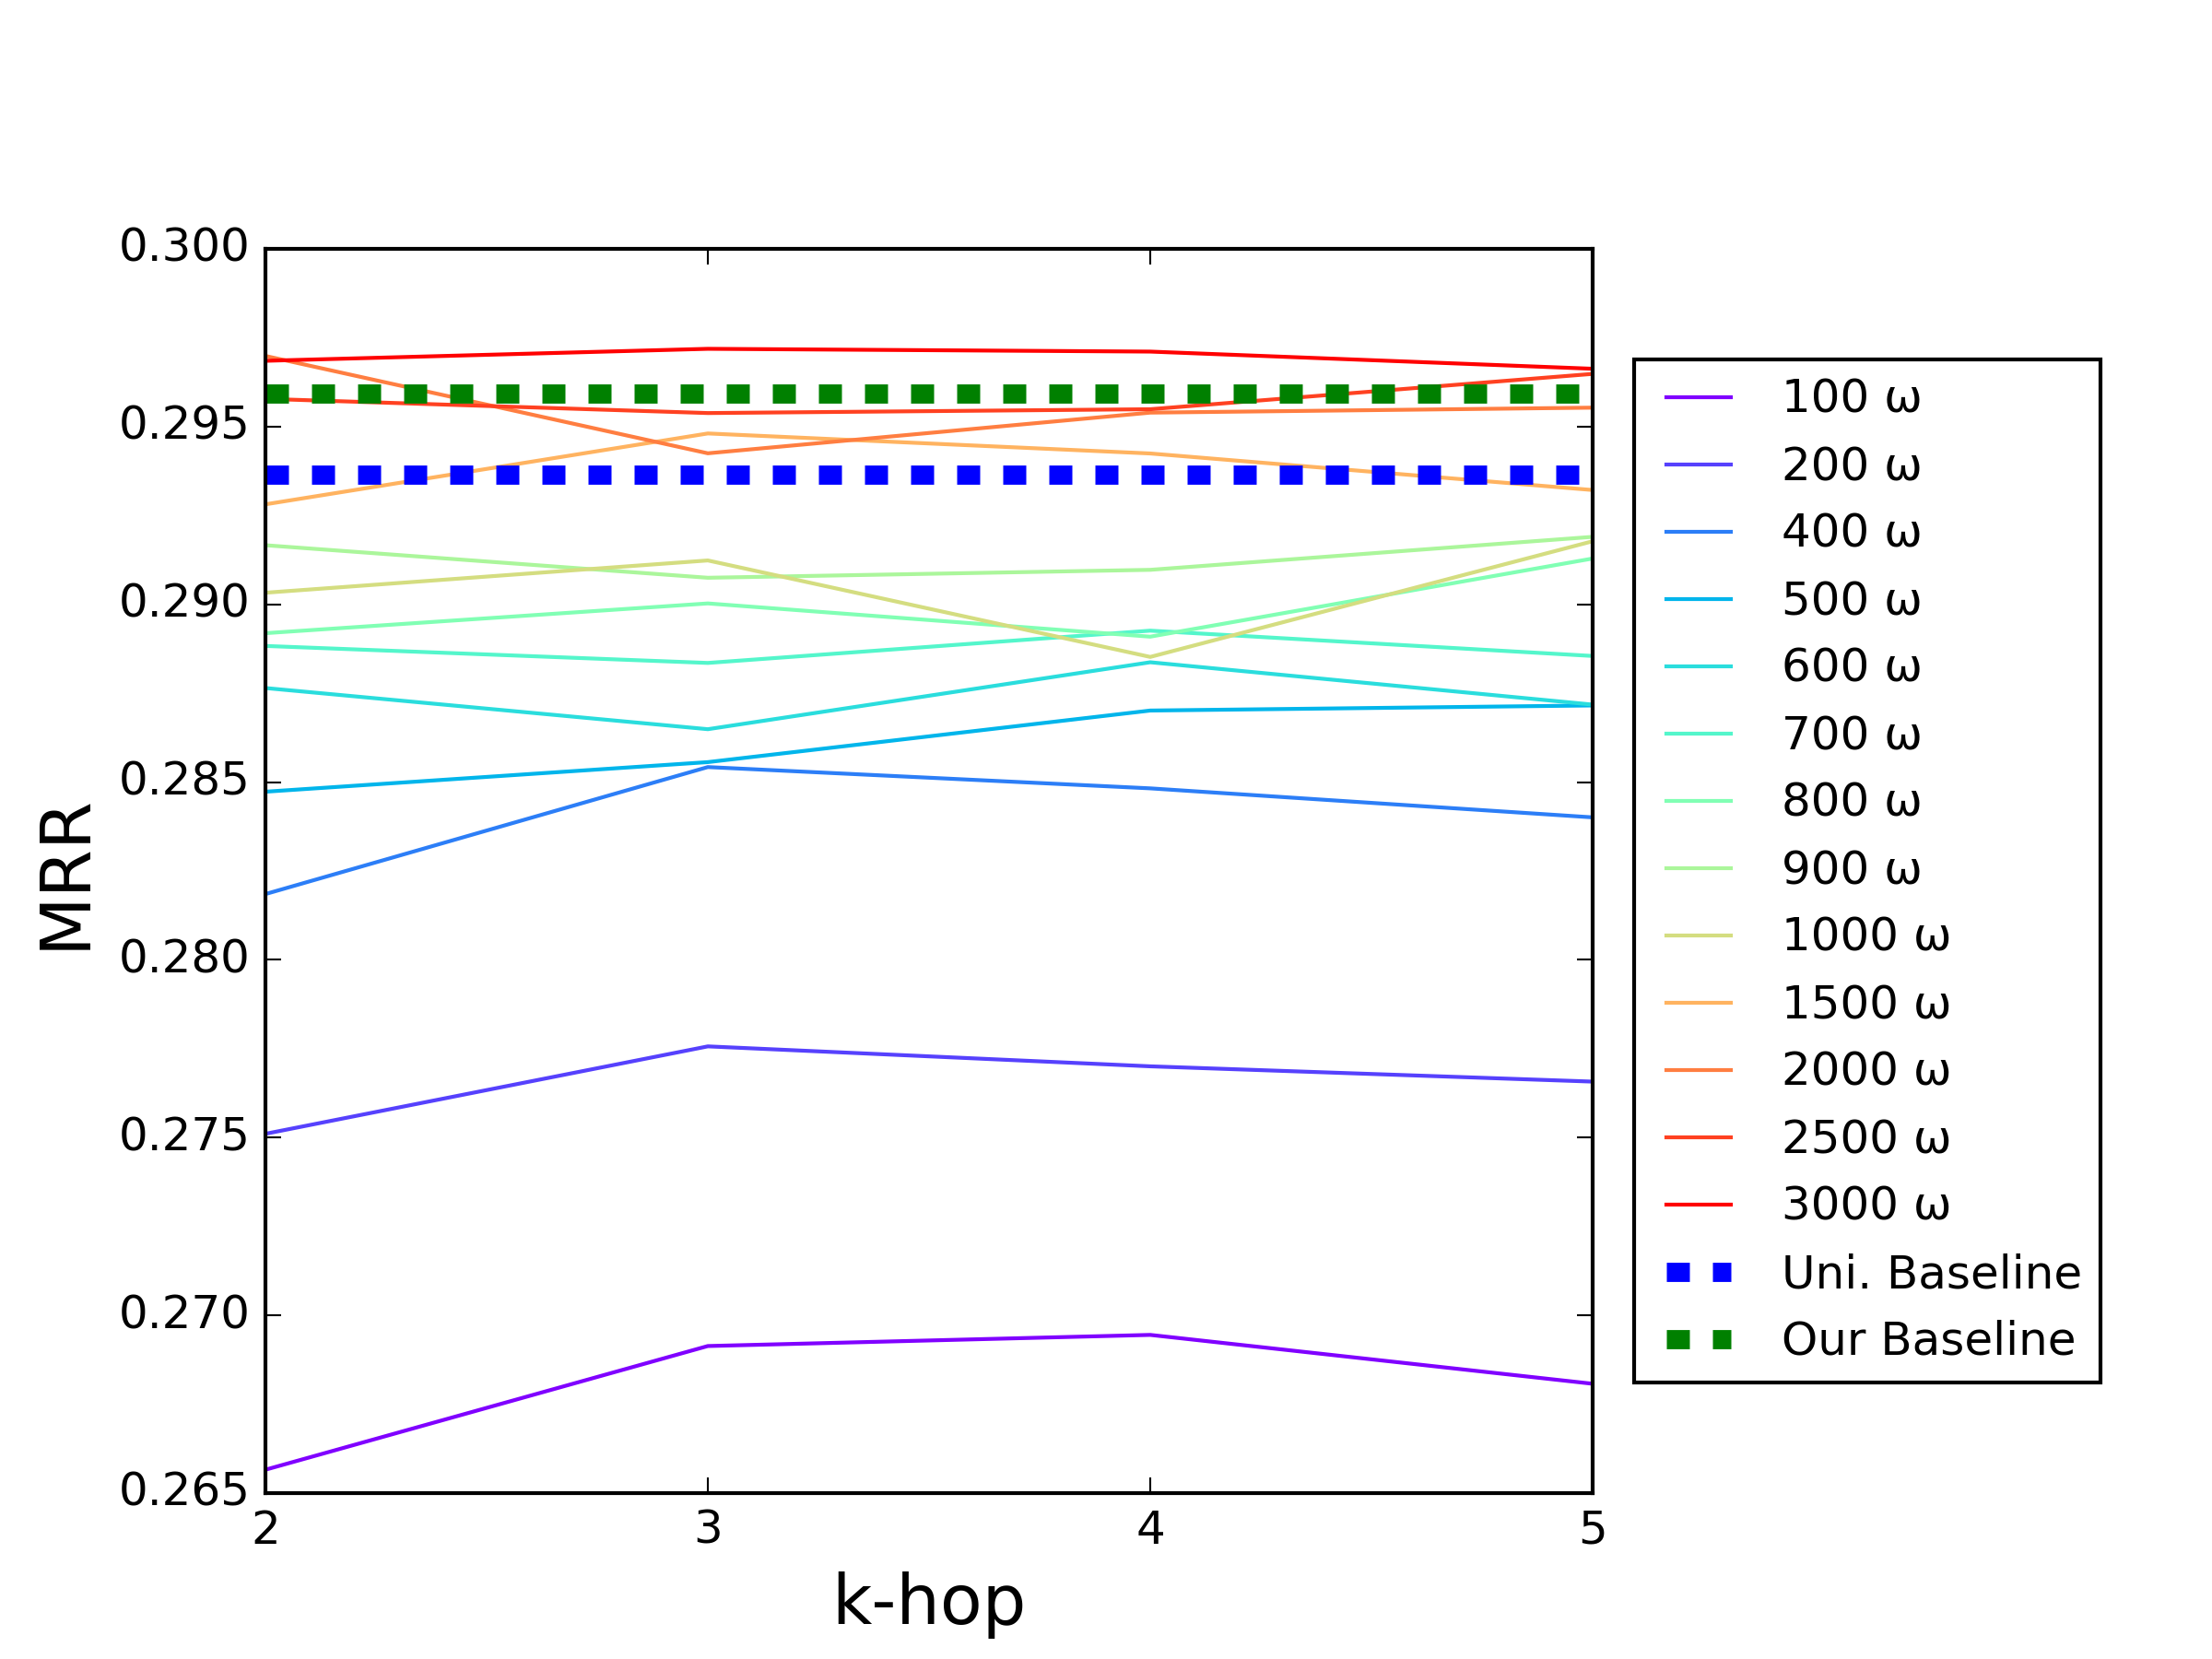
\includegraphics[width=2.5in]{writeup/Results/Ablation.png}
    \caption{The effect of the number of random walks
     for Uniform SANS with the TransE on FB 15k-237.}
    \label{fig:ablation}
\end{figure}
}
% ------------------------------------------------------------------------
% MAIN RESULTS TABLE START

\begin{table*}[h]
\begin{small}
\centering
\begin{tabular}{cccccccc}
\hline
\multirow{3}{2cm}{\centering Score Function}& \multirow{3}{2cm}{Algorithm} & \multicolumn{2}{c}{FB15K-237} & \multicolumn{2}{c}{WN18} & \multicolumn{2}{c}{WN18RR} \\
& & Hit@10 & \multirow{2}{1cm}{\centering MRR} & Hit@10 & \multirow{2}{1cm}{\centering MRR} & Hit@10 & \multirow{2}{1cm}{\centering MRR} \\ 
& & (\%) & & (\%) & & (\%) & \\
\hline
% TransE --------------------------------------------------
\multirow{5}{1.5cm}{\centering TransE} & Uniform \cite{sun2019rotate} & 48.03 & 0.2927 & \textbf{95.53} & 0.6085 & 49.63 & 0.2022 \\
& KBGAN \cite{cai2017kbgan} & 46.59 & 0.2926 & 94.80 & 0.6606 & 45.39 & 0.1808 \\
& IGAN \cite{wang2018incorporating} & - & - & 92.7 & - & - & -\\
& NSCaching \cite{zhang2019nscaching} & 47.64 & 0.2993 & 94.63 & 0.7818$^\dagger$ & 47.83 & 0.2002\\
& Self-Adv. \cite{sun2019rotate} & \textbf{52.73} & \textbf{0.3296} & 92.02 & 0.7722 & 52.78 & 0.2232 \\
& Uniform SANS (ours) & 48.73 & 0.2971 & 95.22$^\dagger$ & \textbf{0.8195} \\
& Self-Adv. SANS (ours) & 50.04$^\dagger$ & 0.3060$^\dagger$ & 88.51 & 0.7429 \\
\hline
% DistMult --------------------------------------------------
\multirow{4}{1.5cm}{\centering DistMult} & Uniform & 40.26 & 0.2537 & 81.39  & 0.4689 & 52.86 & 0.3938 \\
& KBGAN & 39.91 & 0.2272 & 93.08$^\dagger$ & 0.7275$^\dagger$ & 44.32 & 0.3849 \\
& NSCaching & 45.56 & 0.2834 & \textbf{93.74} & \textbf{0.8306} & 45.80 & 0.4148\\
& Self-Adv. & \textbf{48.41} & \textbf{0.3091} & 92.94  & 0.6837 & 53.80 & 0.4399 \\
& Uniform SANS (ours) & 41.46 & 0.2621 & 89.80 & 0.6234 \\
& Self-Adv. SANS (ours) & 48.07$^\dagger$ & 0.3058$^\dagger$ & 91.08  & 0.6633 \\
\hline
% RotatE --------------------------------------------------
\multirow{3}{1cm}{\centering RotatE} & Uniform & 47.85 & 0.2946 & \textbf{96.09} & 0.9474 & 56.51 & 0.4711 \\
& Self-Adv. & \textbf{53.03} & \textbf{0.3362} & 96.05$^\dagger$ & \textbf{0.9498} & 57.29 & 0.4760 \\
& Uniform SANS (ours) & 48.47 & 0.3003 & \textbf{96.09} & 0.9496$^\dagger$ \\
& Self-Adv. SANS (ours) & 51.07$^\dagger$ & 0.3161$^\dagger$ & 96.05$^\dagger$ & \textbf{0.9498} \\
\hline
\end{tabular}
\caption{Comparison of different negative sampling algorithms. Results for KBGAN and NSCaching are taken from \cite{zhang2019nscaching}. IGAN results are taken from \cite{wang2018incorporating}. 
All other results were are taken from our re-implementations. Bold numbers are the best performance, whereas those marked by $\dagger$ are the second-best. 
}
\label{tab:comparison}
\end{small}
\end{table*}

% MAIN RESULTS TABLE END
% ------------------------------------------------------------------------

% % % ------------------------------------------------------------------------
% % of filled entries
\begin{table}[b]
\centering
\begin{tabular}{cccccc}
\hline
$k$ & 2 & 3 & 4 & 5 \\ 
\hline
FB15K-237 & 34 & 83 & 97 & 99 \\
\hline
WN18 & 0.19 & 0.75 & 3.22 & 10.2 \\
\hline
WN18RR & - & - & - & - \\
\hline
\end{tabular}
\caption{Percentage (\%) of the k-hop adjacency tensor that is filled.}
\label{tab:percentage}
\end{table}
% % % ------------------------------------------------------------------------

Table \ref{tab:comparison} is indicative of the best performances achieved while deploying different negative sampling algorithms to train different graph embedding models. As seen, our Uniform SANS performs better than uniform sampling by constraining negative sampling to the \emph{k-hop} neighbourhood. Moreover, our Self-Adversarial SANS performs better than GAN-based and cache-based methods, and exhibits similar performance to the Self-Adversarial technique proposed in \cite{sun2019rotate}. Therefore, our experimental findings suggest that both of our negative sampling algorithms are simple yet effective NEG techniques, with comparable performances to the state-of-the-arts. Most notably, our NEG algorithms require less computational resources for using a smaller distribution of negative triplets. This is verified by Table \ref{tab:percentage}, where the percentage of filled entries in the \emph{k-hop} adjacency tensor have been listed. 

Lastly, comparing the results obtained with our Uniform SANS scheme to the ones achieved by NSCaching, which uses high quality negative triplets, indicated that nodes within close proximity to each other may create ``hard'' negative examples, which supports our initial hypothesis. A more detailed set of experimental findings, presenting the performance of our negative sampling algorithms against uniform sampling and self-adversarial sampling with different hyperparameters, as well as information regarding their space and time complexity can be found in \ref{sec:supplemental}.

% --------------------------------------------------------------------------------------------------------------------

\cut{
Additionally, Table \ref{tab:times} compares the time and space complexity of different NEG algorithms, which emphasize the cheapness of their runtime and space complexities compare to the state-of-the-arts. 

Lastly, Table \ref{tab:percentage} also shows the percentage of filled entries in the \emph{k-hop} adjacency matrix, that is informative of the size of the subspace from which negative examples are drawn from. With regards to these values, our NEG algorithm uses a smaller negative sampling subspace compared to the standard NEG approaches, yet demonstrates comparable performance. A more detailed set of results, presenting the performance of our NEG algorithms against uniform sampling and self-adversarial sampling with different hyperparameters, can be found in our supplementary document.
}

\section{Conclusion and Future Directions}
\label{sec:conclusion}

In this work, we proposed two novel negative sampling approaches, namely Uniform SANS and Self-Adversarial SANS, which leverage information about local neighborhood structures, namely the \emph{k-hop} neighbourhood of a node, to select negative examples. According to our findings, the comparable performance of our negative sampling approach to the state-of-the-arts emphasized the importance of accounting for underlying graph structure while selecting negative examples. Respectfully, it would be worthwhile to extend the idea of structural negative sampling in various ways for efficient and effective training of graph embedding models. A potential improvement could be training graph embedding models with positive and negative context graphs \cite{navarin2018pre} in addition to positive and negative triplets.



% As future directions, the idea of structural NEG can be taken further by training graph embedding models with positive and negative triplets as well as positive and negative context graphs \cite{navarin2018pre}. Lastly, one can extend the idea used in GAN-based NEG methods by finding the worst case negative triplet from a ball of radius $R$, and minimize the loss function with respect to it. The added benefit of using such \emph{robust} NEG scheme compared to the GAN-based ones is eliminating the need for a generator to create negative examples.  

% We propose two techniques which take the idea of structural NEG further. As done in   \cite{navarin2018pre}, context graphs can be used to pre-train Graph Neural Networks (GNNs) at node level to improve transfer learning, by enabling prediction of the surrounding graph structure. Similarly, this idea can be implemented in structural NEG to train graph embedding models with positive and negative triplets as well as positive and negative context graphs. In this scheme, positive examples are sub-graphs that share the same center node, and negative examples are the ones with different nodes as their center node which may or may not lie within the \emph{k-hop} neighbourhood. Lastly, one can extend the idea used in GAN-based NEG methods by finding the worst case negative triplet from a ball of radius $R$, and minimize the loss function with respect to it. The added benefit of using such \emph{robust} NEG scheme compared to the GAN-based ones is eliminating the need for a generator to create negative examples.  




% \section*{Acknowledgments}

% The acknowledgments should go immediately before the references. Do not number the acknowledgments section.
% Do not include this section when submitting your paper for review.

\clearpage

\bibliography{anthology,emnlp2020}
\bibliographystyle{acl_natbib}


% -------------------------------------------------------
\newpage

\appendix

\onecolumn

% \section{Appendices}
\label{sec:appendix}

\newpage
\section{Supplemental Material}
\label{sec:supplemental}

% % ------------------------------------------------------------------------
% COMPLEXITY TABLE START

\begin{table}[!htbp]
    \centering
    \begin{tabular}{cccc}
    \hline
         \multirow{2}{3cm}{\centering NEG Algorithm} & Preprocessing  & Runtime  & Space \\
         & Complexity & Complexity & Complexity
         \\
         \hline
         Uniform \cite{bordes2013translating} & $O(1)$ & $O(bn)$ & $O(1)$ \\
         IGAN \cite{yu2014improving} & $O(t)$ & $O(bnt + bt)$ & $O(t)$ \\
         KBGAN \cite{cai2017kbgan} & $O(t)$ & $O(bn + bd + bt)$ & $O(t)$ \\
         NSCaching \cite{zhang2019nscaching} & $O(1)$ & $O(bn + be)$ & $O(c|R||V|)$ \\
         Self-Adv. \cite{sun2019rotate} & $O(|E|)$ & $O(bn + bd)$ & $O(|E|)$ \\
         Structural Uni. (ours) & $O(|V|^3\log k)$ & $O(bn)$ & $O(|V|^2)$ \\
         Structural Adv. (ours) & $O(|V|^3\log k)$ & $O(bn + bd)$ & $O(|V|^2)$ \\
         Structural RW Uni. (ours) & $O(rk|V|)$ & $O(bn)$ & $O(r|V|)$ \\
         Structural RW Adv. (ours) & $O(rk|V|)$ & $O(bn + bd)$ & $O(r|V|)$ \\
         \hline
    \end{tabular}
    \caption{Comparison of different negative sampling algorithms in terms of preprocessing, runtime, and space complexities given batch size $b$, negative sample size $n$, cache size $c$, cache extension size $e$, node set $V$, edge set $E$, relation set $R$, embedding dimension $d$, hops count $k$, random walks count $r$, and GAN parameters count $t$.}
    \label{tab:times}
\end{table}

% COMPLEXITY TABLE END
% % ------------------------------------------------------------------------

 \end{document}
